\chapter{电磁学}

\newpage
{\bf 这里是一段关于电磁学的介绍。}

\newcommand\resistance{
	\begin{tikzpicture}[baseline = {([yshift = -3.5pt] current bounding box.center)}]
		\draw (0, 0) rectangle (0.6, 0.2);
		\draw (-0.3, 0.1) -- (0, 0.1);
		\draw (0.6, 0.1) -- (0.9, 0.1);
	\end{tikzpicture}
}

\newcommand\ammeter{
	
\begin{tikzpicture}[baseline = {([yshift = -3.5pt] current bounding box.center)}]
		\node (A) [circle, draw, scale = 1, inner sep = 1pt, line width = 0.5pt] at (0, 1){\small A};
	\end{tikzpicture}
} % ~{\Large\textcircled{\small A}}~

\newcommand\voltmeter{
	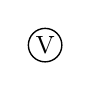
\begin{tikzpicture}[baseline = {([yshift = -3.5pt] current bounding box.center)}]
		\node (V) [circle, draw, scale = 1, inner sep = 1pt, line width = 0.5pt] at (0, 1){\small V};
	\end{tikzpicture}
} % ~{\Large\textcircled{\small V}}~

\newcommand\slidingrheostat{
	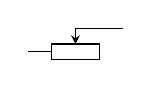
\begin{tikzpicture}[baseline = {([yshift = -3.5pt] current bounding box.center)}]
		\draw (0, 0) rectangle (0.6, 0.2);
		\draw (-0.3, 0.1) -- (0, 0.1);
		\draw [-stealth] (0.3, 0.4) -- (0.3, 0.2);
		\draw [line join = miter] (0.9, 0.4) -- (0.3, 0.4) -- (0.3, 0.3);
	\end{tikzpicture}
}

\section{电荷}

\vspace{10pt}
\begin{itemize}
\item 物体能够吸引轻小物体,就说物体带了电,即物体带了\blue{电荷}(electric charge)。带了电荷的物体叫做\blue{带电体}。
\item 使物体带电叫做\blue{起电}。用摩擦的方式使物体带电叫做\blue{摩擦起电}(electrification by friction)。
\item 自然界\blue{只有}两种电荷。
\item 用丝绸摩擦过的玻璃棒带的电荷叫做\blue{正电荷}(positive charge)。用毛皮摩擦过的橡胶棒带的电荷叫做\blue{负电荷}(negative charge)。
\item \blue{同种}电荷相互\blue{排斥},\blue{异种}电荷相互\blue{吸引}。
\item 电荷的多少叫做\blue{电荷量}(electric quantity),简称\blue{电量}。用 \blue{$\bm Q$} 或 \blue{$\bm q$} 表示。在国际单位制中,电荷量的单位是\blue{库仑}(coulomb),简称\blue{库}。符号是 \blue{$\bf C$}。正电荷的电荷量为正值,负电荷的电荷量为负值。
\item \blue{验电器}和\blue{静电计}。
\item 两种电荷互相完全抵消叫做\blue{中和}。
\item 物质是由\blue{分子}构成的,分子是由\blue{原子}构成的。
\item 原子是由带正电的\blue{原子核}和带负电的\blue{电子}(electron)组成的。
\item 原子核是由带正电的\blue{质子}和不带电的\blue{中子}组成的。
\item 每个原子中质子与电子的\blue{数量相等},质子与电子所带的\blue{电荷量相同}。
\item 摩擦起电的本质是电荷从一个物体\blue{转移}到另一个物体。
\item 金属原子中能脱离原子核的束缚而在金属中自由运动的电子叫做\blue{自由电子}(free electron)。
\item 失去自由电子的原子叫做\blue{离子}(ion)。
\item 质子、电子所带的电荷量(\blue{最小的电荷量})叫做\blue{元电荷}(elementary charge),用 \blue{$\bm e$} 表示。有:
\mathline{e\approx1.6\times10^{-19}\text{C}}
\item 所有带电体的电荷量都是 $e$ 的整数倍,不是连续变化的,即量子化的。
\item 电子的电荷量 $e$ 与质量 $m_e$ 之比叫做\blue{电子的比荷}(specific charge)。电子的质量 $m_e=9.11\times10^{-31}\text{kg}$,则电子的比荷为:
$$
\frac{e}{m_e}\approx1.76\times10^{11}\text{C}/\text{kg}
$$
\item 利用静电感应使金属带电叫做\blue{感应起电}(electrification by induction),所带电荷叫做\blue{感应电荷}(induced charge)。
\item \blue{静电感应}(electrostatic induction)。
\item 三种常见的起电方式包括摩擦、接触、感应。
\item \blue{电荷守恒定律}(law of conservation of charge),即电荷既不会创生,也不会消灭。它只能从一个物体转移到另一个物体,或者从物体的一部分转移到另一部分。在转移的过程中,电荷的总量保持不变。
\item 一个与外界没有电荷交换的系统,电荷的\blue{代数和}保持不变。
\item 电荷守恒定律是自然界最普遍、最重要的基本定律之一。
\end{itemize}
\newpage
\section{电路}

\subsection{简单电路}
\vspace{10pt}
\begin{itemize}
\item \blue{电路}(electric circuit),即用导线、用电器、开关连接起来.
\item \blue{电源}(power supply),即提供电能的装置,如电池、发电机.
\item \blue{用电器},即消耗电能的装置,如灯泡、电动机.
\item \blue{开关},即控制电路通断的装置,如单刀单掷开关、单刀双掷开关.
\item \blue{导线}通常由绝缘外皮和金属内芯(铜或铝)组成.
\item 处处连通的电路叫做\blue{通路}(\blue{闭合电路}). 某处断开的电路叫做\blue{断路}(\blue{开路}).
\item \blue{直接}用导线将电源的正、负极连接起来的电路叫做\blue{短路}.
\item 闭合电路中,用电器两端被导线直接连通叫做用电器被\blue{短接}.
\item 用符号表示电路连接的图叫做\blue{电路图}.
\item \blue{串联}(series connection)合\blue{并联}(parallel connection).
\item \blue{串联电路}和\blue{并联电路}.
\item 串联电路中各用电器相互影响,并联电路各用电器互不影响.
\end{itemize}
\section{欧姆定律}

\subsection{电流与电压、电阻的关系}
\begin{itemize}
\item 在\blue{电阻一定}时,通过导体的电流与导体两端的电压成正比.
\item 在\blue{电压一定}时,通过导体的电流与导体的电阻成正比.
\item \blue{欧姆定律}(Ohm's law),即导体中的电流,跟导体两端的电压成正比,跟导体的电阻成反比. 有:
\mathline{I=\frac UR}
\newline 欧姆定律对金属、电解液适用,对半导体、电离气体不适用.
\end{itemize}

\subsection{电阻的测量}
\begin{itemize}
\item 伏安法测电阻,即利用 $R=\frac UI$ 测量电阻.
\item 小灯泡是非线性元件,其伏安特性曲线如图.
\begin{figure}[H]
	\centering
	\begin{tikzpicture}
	\begin{axis}[
		axis lines = middle,
		xmin = 0, xmax = 10,
		ymin = 0, ymax = 10,
		smooth, thick,
		xlabel = {$U/\text{V}$}, ylabel = {$I/\text{A}$},
		xlabel style = {anchor = north},
		ylabel style = {anchor = east},
		xtick = \empty,	ytick = \empty,
		samples = 200,
	]
		\addplot+[no marks, domain = 0 : 10]{log10(x + 1) / log10(1.35)};
	\end{axis}
	\node at (0, 0) [below = 5pt, left = -2pt] {$O$};
	\end{tikzpicture}
	\titlename{小灯泡的伏安特性曲线}
\end{figure}
\end{itemize}

\subsection{串、并联电路中的分压、分流规律}
\begin{itemize}
\item 串联分压,即 \blue{$\bm{U_1:U_2:\cdots:U_n=R_1:R_2:\cdots:R_n}$}.
\item 并联分流,即 \blue{$\bm{I_1:I_2:\cdots:I_n=\frac1{R_1}:\frac1{R_2}:\cdots:\frac1{R_n}}$}.
\end{itemize}
\section{电功和电功率}

\subsection{电功和电能}
\begin{itemize}
\item \blue{电能}(electric energy)可以转化为其他形式的能. 单位是\blue{焦耳},简称\blue{焦},符号是 \blue{$\bf J$}. 常用单位还有\blue{千瓦时},简称\blue{度},符号是 \blue{$\bf kW\cdot h$}. 换算关系是 \blue{$\bf 1kW\cdot h=3.6\times10^6J$}.
\item 电流做的功叫做\blue{电功}(electric work). 用 \blue{$\bm W$} 表示. 单位是\blue{焦耳},简称\blue{焦},符号是 \blue{$\bf J$}.
\item 电流做了多少功,就有多少电能转化为其他形式的能.
\item 电功等于电压 $U$、电流 $I$ 和通电时间 $t$ 的乘积,即:
\mathline{W=UIt}
\item 根据 $U=IR$,电流通过电阻 $R$ 做的功为:
$$
W=I^2Rt~~或~~W=\frac{U^2}Rt
$$
\item 电功或电能的计量仪器叫做\blue{电能表}(电度表).
\end{itemize}

\subsection{电功率}
\begin{itemize}
\item \blue{电功率}(electric power)是表示\blue{电能做功快慢}的物理量. 用 \blue{$\bm P$} 表示. 单位是\blue{瓦特},简称\blue{瓦},符号是 \blue{$\bf W$}. 常用单位还有千瓦(\blue{$\bf kW$})、毫瓦(\blue{$\bf mW$}). 换算关系是 \blue{$\bf1kW=10^3W$},\blue{$\bf1mW=10^{-3}W$}.
\item 电功率等于电流 $U$ 和电压 $I$ 的乘积,即:
\mathline{P=\frac Wt=UI}
\item 根据 $U=IR$,电流通过电阻 $R$ 的电功率为:
$$
P=I^2R~~或~~P=\frac{U^2}R
$$
\item 用电器正常工作时的电压叫做\blue{额定电压}(rated voltage),用电器在额定电压下工作时的电功率叫做\blue{额定功率}(rated power).
\end{itemize}
\section{磁}

\subsection{磁现象}
\Itemize{
\item 能够吸引\blue{铁}、\blue{钴}、\blue{镍}等物质的性质叫做\Keyword{磁性}{magnestion}。
\item 具有磁性的物体叫做\Keyword{磁体}{magnet}。
\item 磁性最强的两个部位叫做\Keyword{磁极}{magnetic pole}。
\item 能够自由转动的磁体,静止时由指向北方的磁极叫做\Keyword{北极}{north pole}或 \blue{N 极},指向南方的磁极叫做\Keyword{南极}{south pole}或 \blue{S 极}。
\item 磁极间相互作用的规律,即\blue{同名磁极相互排斥},\blue{异名磁极相互吸引}。
\item 原本没有磁性的物体在磁体或电流的作用下获得磁性的过程叫做\Keyword{磁化}{magnestization}。
\item 能够被磁化的物质统称为\blue{磁性材料}。
\item 磁性材料分为硬磁性材料和软磁性材料。
\item 被磁化后能够长期保持磁性的材料叫做\blue{硬磁性材料}(永磁体)。被磁化后不能长期保持磁性的材料叫做\blue{软磁性材料}。
}

\subsection{磁场}
\Itemize{
\item \Keyword{磁场}{magnestion field}的\blue{基本性质},即磁场对放入其中的磁体有力的作用。
\item 磁场中的不同位置磁场的强弱和方向不同。
\item \blue{规定}小磁针静止时 \blue{N 极所指的方向}为这点磁场的方向。
\item \Keyword{磁感线}{magnetic induction line}\blue{不存在},只是为了方便形象地描述磁场。
\item 磁体外部的磁感线都是从磁体的 \blue{N 极出发回到 S 极}。
\item \blue{磁感线疏密表示磁场强弱}。磁感线稀疏的地方磁场弱,磁感线密集的地方磁场强。
\item 磁感线上某点的\blue{切线方向},既是放在该处的小磁针 \blue{N 极的受力方向},也是该点的\blue{磁场方向}。
\item 地球周围空间存在的磁场叫做\blue{地磁场}。
\item 地磁的 N 极在地理的南极附近,地磁的 S 极在地理的北极附近。
\item 地磁场的两级和地理的两级不重合。
\item 地磁场的磁感线分布跟条形磁体的磁场相似。
\item 磁针所指南北方向偏离地理南北方向的角度叫做\blue{磁偏角}。
}

\subsection{电流的磁感应}
\Itemize{
\item 奥斯特实验。
\item 通电导线周围存在与电流方向有关的磁场,这种现象叫做\blue{电流的磁效应}。
\item 通电\blue{螺线圈}(\blue{线圈})外部的磁场与条形磁体的磁场相似。
\item \Keyword{安培定则}{Anpere's rule}或\Keyword{右手螺旋定则}{right-handed screw rule}。
}

\subsection{电磁铁及其应用}
\Itemize{
\item \Keyword{电磁铁}{electromagnet},即\blue{线圈}与\blue{铁芯}的组合。
\item 有电流时产生磁性,没有电流时失去磁性。
\item 匝数一定时,\blue{电流}越大,电磁铁的磁性越强。电流一定时,\blue{匝数}越多,电磁铁的磁性越强。
\item \blue{继电器}是利用低电压、弱电流电路的通断,来间接地控制高电压、强电流电路通断的装置。
\item \blue{电磁继电器}是利用电磁铁来控制工作电路的一种开关。其工作电路由\blue{低压控制电路}和\blue{高压工作电路}两部分构成。
}

\subsection{安培力与电动机}
\Itemize{
\item 通电导线在磁场中受到力的作用,力的方向跟电流的方向、磁场的方向有关,这个力叫做\blue{安培力}。
\item \Keyword{左手定则}{left-hand rule}。
\item 电动机是将电能转化为其他形式能的装置。
\item 电动机分为\blue{直流电动机}和\blue{交流电动机}。
\item 电动机由转子和定子两部分组成。能够转到的部分(线圈)叫做\blue{转子},固定不动的部分(磁体)叫做\blue{定子}。
}

\subsection{电磁感应与发电机}
\Itemize{
\item \blue{闭合电路}的\blue{一部分导体}在磁场中做\blue{切割磁感线}运动时,导体中就产生电流,这种现象叫做\Keyword{电磁感应}{electromagnetic induction}。产生的电流叫做\Keyword{感应电流}{induction current}。
\item \Keyword{右手定则}{right hand rule}。
\item 发电机是将其他形式能转化为电能的装置。
\item 发电机分为\blue{直流发电机}和\blue{交流发电机}。
\item 发电机由\blue{转子}(转动部分)和\blue{定子}(固定部分)两部分组成。
\item 方向随时间变化的电流叫做\Keyword{交变电流}{alternating current},简称\blue{交流},符号 \blue{AC}。方向不随时间变化的电流叫做\Keyword{直流电流}{direct current},简称\blue{直流},符号 \blue{DC}。
\item 交变电流的频率在数值上等于电流在每秒内周期性变化的次数。
\item 我国电网以交流供电,频率为 \blue{50Hz}。
}